\section{Experiments}
\label{sec:experiments}

\subsection{Setup}

\paragraph{Instances.}
Eight synthetic configurations spanning 10--100 scenes (Table~\ref{tab:instances}), generated with fixed seed~42.
Parameters follow established literature ranges~\citep{bomsdorf2008}: wages \$80--\$1{,}000/day, 20\% precedence probability, 80\% actor availability, hierarchical transfer costs \$100--\$8{,}000 (by geographic tier).
All 19 constraint families are active in every instance.

\begin{table}[t]
\centering
\caption{Instance configurations: $|\mathcal{S}|$ scenes, $|\mathcal{A}|$ actors,
         $|\mathcal{C}|/|\mathcal{I}|/|\mathcal{L}|$ cities/towns/locations,
         $T$ planning days, and $K$ SIG blocks.}
\label{tab:instances}
\small
\begin{tabular}{@{}lcccccc@{}}
\toprule
\textbf{Config} & $|\mathcal{S}|$ & $|\mathcal{A}|$ & $|\mathcal{C}|/|\mathcal{I}|/|\mathcal{L}|$ & $T$ & $K$ \\
\midrule
S10  & 10  & 5   & 1/2/3   & 15  & 4  \\
S15  & 15  & 8   & 1/2/4   & 25  & 3  \\
S20  & 20  & 10  & 2/3/5   & 35  & 6  \\
S25  & 25  & 12  & 2/4/6   & 45  & 8  \\
S30  & 30  & 15  & 2/4/7   & 55  & 8  \\
S50  & 50  & 20  & 3/6/10  & 90  & 14 \\
S75  & 75  & 35  & 4/8/12  & 120 & 17 \\
S100 & 100 & 43  & 5/10/15 & 150 & 26 \\
\bottomrule
\end{tabular}
\end{table}

\paragraph{Algorithms.}
\textbf{BDM-AOS}: population~20, generations~40, $p_c{=}0.9$, $p_m{=}0.3$.
\textbf{GA}: population~50, 100~generations, OX crossover, $p_c{=}0.85$, $p_m{=}0.15$~\citep{goncalves2011}.
\textbf{PSO}: swarm~30, 100~iterations, $w{=}0.7$, $c_1{=}c_2{=}1.5$~\citep{kennedy1995}.
\textbf{MILP}: CBC solver, 300\,s time limit.
Each metaheuristic is run with 30 independent random seeds.
Five ablation variants isolate individual BDM components: BDM-NoAOS, BDM-NoSpecOps, BDM-Flat, BDM-NoSIG.

\paragraph{MILP comparison.}
BDM-AOS matches MILP optimality on S10 (both \$12.5k; $19\times$ faster: 0.20\,s vs.\ 3.8\,s) and is within 4\% of optimal on S15 ($129\times$ faster).
For $n \geq 20$, MILP exhausts its 300\,s budget without proving optimality (integrality gap 22--39\%); for $n \geq 30$, MILP finds no feasible solution at all.
BDM-AOS solves every instance in under 2\,seconds regardless of scale---a ${>}186\times$ runtime advantage at S100.

\subsection{Main Results}

\begin{table}[t]
\centering
\caption{Mean cost (\$k) / mean runtime (s) over 30 seeds.
         \textbf{Bold} = best mean cost among metaheuristics for that instance.}
\label{tab:results}
\small
{\setlength{\tabcolsep}{4pt}
\begin{tabular}{@{}lcccccc@{}}
\toprule
\textbf{Alg.} & \textbf{S10} & \textbf{S20} & \textbf{S30}
              & \textbf{S50} & \textbf{S75} & \textbf{S100} \\
\midrule
GA      & \textbf{12.5}/0.34 & 33.4/0.81          & \textbf{37.4}/1.53
        & 113.0/3.51         & 169.6/6.16         & 272.1/8.78 \\
PSO     & \textbf{12.5}/0.19 & \textbf{32.5}/0.47 & 40.1/0.94
        & \textbf{112.8}/2.11 & 166.0/3.56        & 265.5/5.23 \\
BDM-AOS & \textbf{12.5}/0.20 & 40.3/0.28          & 49.8/0.41
        & 119.1/0.71         & \textbf{134.5}/1.10 & \textbf{232.8}/1.61 \\
\bottomrule
\end{tabular}}
\end{table}

Results (Table~\ref{tab:results}, Figure~\ref{fig:scalability}) show a clear scalability crossover (see block counts $K$ in Table~\ref{tab:instances}).
On small--medium instances (S10--S30, $K{=}3$--$8$), GA and PSO outperform BDM-AOS because the block-permutation space is too coarse relative to the full scene space.
At S50 ($K{=}14$) the gap narrows to 5.6\%.
At S75 ($K{=}17$), BDM-AOS \textbf{outperforms both baselines by 20.7\% and 19.0\%} while running $5.6\times$ faster.
At S100 ($K{=}26$), BDM-AOS maintains a \textbf{14.5\%} cost advantage over GA at $5.5\times$ speedup.
Wilcoxon rank-sum tests (Holm-corrected, $\alpha{=}0.05$): BDM-AOS significantly outperforms both GA and PSO on S75 and S100 ($p < 0.001$).

\begin{figure}[t]
\centering
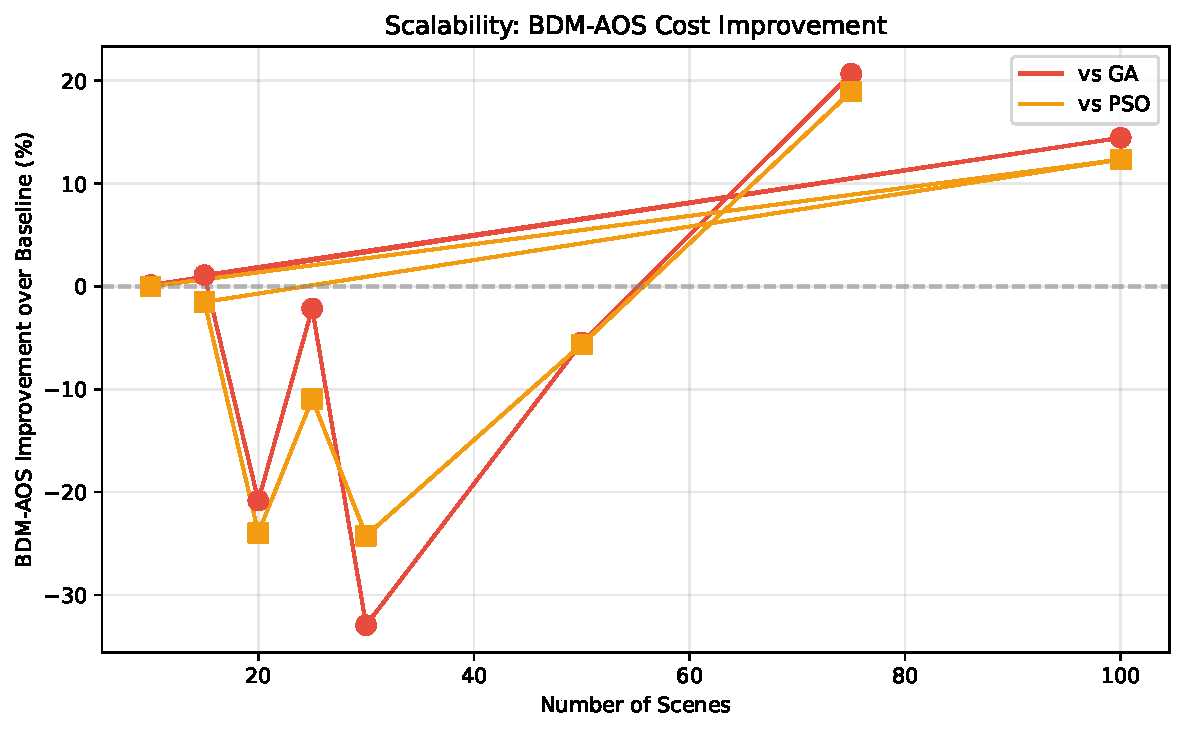
\includegraphics[width=0.52\textwidth]{figures/scalability_improvement.pdf}
\caption{Relative cost gap of BDM-AOS vs.\ the best baseline (GA or PSO).
         Negative values indicate BDM-AOS achieves lower cost.
         The crossover occurs between S50 and S75.}
\label{fig:scalability}
\end{figure}

\subsection{Ablation Study}

\begin{table}[t]
\centering
\caption{Ablation study: mean cost (\$k) and degradation $\Delta$\% relative to BDM-AOS (full), averaged over 30 seeds.}
\label{tab:ablation}
\small
\begin{tabular}{@{}lrrrrrr@{}}
\toprule
 & \multicolumn{2}{c}{\textbf{S50}}
 & \multicolumn{2}{c}{\textbf{S75}}
 & \multicolumn{2}{c}{\textbf{S100}} \\
\cmidrule(lr){2-3}\cmidrule(lr){4-5}\cmidrule(lr){6-7}
\textbf{Variant}
  & \textbf{Mean} & \textbf{$\Delta$\%}
  & \textbf{Mean} & \textbf{$\Delta$\%}
  & \textbf{Mean} & \textbf{$\Delta$\%} \\
\midrule
BDM-AOS (full)   & \textbf{119.1} & ---   & \textbf{134.5} & ---   & \textbf{232.8} & ---   \\
BDM-NoAOS        & 121.1          & +1.7  & 137.2          & +2.0  & 233.0          & +0.1  \\
BDM-NoSpecOps    & 120.7          & +1.3  & 175.4          & +30.4 & 233.2          & +0.2  \\
BDM-Flat         & 129.4          & +8.6  & 215.1          & +59.9 & 303.4          & +30.3 \\
BDM-NoSIG        & 158.8          & +33.3 & 221.1          & +64.3 & 328.1          & +41.0 \\
\midrule
GA  (reference)  & 113.0          & $-$5.1 & 169.6         & +26.1 & 272.1          & +16.9 \\
PSO (reference)  & 112.8          & $-$5.3 & 166.0         & +23.4 & 265.5          & +14.1 \\
\bottomrule
\end{tabular}
\end{table}

\textbf{SIG decomposition is critical}: BDM-NoSIG degrades by 33\% on S50, 64\% on S75, and 41\% on S100, confirming that Louvain-guided partitioning captures genuine actor--location coupling.
\textbf{Q-learning AOS} yields modest, scale-dependent gains (1.7--2.0\% on S50--S75), diminishing at S100 as the Q-table state space becomes too coarse for $K{=}26$ blocks.
\textbf{Domain-specific operators} (LAX/ACM) show a pronounced S75 spike (+30.4\%), where block count $K{=}17$ aligns well with their design; the effect diminishes at S100.
\textbf{BDM-Flat} ($K{=}n$ blocks) confirms that intermediate block granularity is optimal: operating at scene level causes 8.6--59.9\% degradation on S50--S75.
